% Dokumentklassen s�ttes til memoir.
% Manual: http://ctan.org/tex-archive/macros/latex/contrib/memoir/memman.pdf
\documentclass[a4paper,oneside,article]{memoir}

\usepackage{pgf}
\usepackage{tikz}
\usepackage{pgfplots}
\usetikzlibrary{arrows,automata}
\usepackage{verbatim}
 
% Danske udtryk (fx figur og tabel) samt dansk orddeling og fonte med
% danske tegn. Hvis LaTeX brokker sig over �, � og � skal du udskifte
% "utf8" med "latin1" eller "applemac". 
\usepackage{inputenc}
\usepackage[danish]{babel}
\usepackage[T1]{fontenc}
 
% Matematisk udtryk, fede symboler, theoremer og fancy ting (fx k�debr�ker)
\usepackage{amsmath,amssymb}
\usepackage{bm}
\usepackage{amsthm}
%\usepackage{mathtools}
 
% Kodelisting. Husk at l�se manualen hvis du vil lave fancy ting.
% Manual: http://mirror.ctan.org/macros/latex/contrib/listings/listings.pdf
\usepackage{listings}
 
% Fancy ting med enheder og datatabeller. L�s manualen til pakken
% Manual: http://www.ctan.org/tex-archive/macros/latex/contrib/siunitx/siunitx.pdf
%\usepackage{siunitx}

% Inds�ttelse af grafik.
\usepackage{graphicx}
\usepackage{float}
\usepackage{caption}
\usepackage{subcaption}
 
% Reaktionsskemaer. L�s manualen for at se eksempler.
% Manual: http://www.ctan.org/tex-archive/macros/latex/contrib/mhchem/mhchem.pdf
%\usepackage[version=3]{mhchem}
%\usepackage[noend]{algpseudocode}
%\usepackage{algorithm}

\usepackage{xcolor,colortbl}

\usepackage{listings}

\definecolor{javared}{rgb}{0.6,0,0} % for strings
\definecolor{javagreen}{rgb}{0.25,0.5,0.35} % comments
\definecolor{javapurple}{rgb}{0.5,0,0.35} % keywords
\definecolor{javadocblue}{rgb}{0.25,0.35,0.75} % javadoc

\lstset{language=Java,
basicstyle=\small, %\ttfamily,
keywordstyle=\color{javapurple}\bfseries,
stringstyle=\color{javared},
commentstyle=\color{javagreen},
morecomment=[s][\color{javadocblue}]{/**}{*/},
numbers=left,
numberstyle=\tiny\color{black},
stepnumber=1,
numbersep=10pt,
tabsize=4,
showspaces=false,
showstringspaces=false}

\newcommand{\notimplies}{%
  \mathrel{{\ooalign{\hidewidth$\not\phantom{=}$\hidewidth\cr$\implies$}}}}

\begin{document}
    \title{Data-Centric Consistency - Disposition}
    \author{Lukas Peter J�rgensen, 201206057, DA4
            }
    \maketitle
    
    \chapter{Terms}
    \begin{itemize}
    \item[Consistency model] A contract between processes and the data store, if processes agree to obey certain rules, the store promises to work correctly.
    \end{itemize}
    
    \chapter{Replicating data}
    Two main reasons for replicating data: \textbf{Reliability} and \textbf{performance}. It becomes reliable because, if one replica crashes, you can just switch to another one, and you can perform on n replicas, and assume that the most common answer is the correct one (in case some doesn't reply the same answer as the other because of corruption).\\
    Performance comes from being able to divide work over multiple servers, or by placing a replica closer to the client (geographically) so the latency is smaller. (Like the Netflix vs Verizon issue).\\
    \\
    \textbf{Cons:}\\
    The cons of replicating data is the trouble with keeping the data consistent.
    
    \chapter{Continuous consistency}
    Distinguish 3 independent axes for defining inconsistencies:
    \begin{enumerate}
    \item Deviation in numerical values between replicas.
    \item Deviation in staleness between replicas.
    \item Deviation with respect to the ordering of update operations.
    \end{enumerate}
    
    \section*{Numerical deviation}
    Useful for when the data have numerical semantics e.g. stock market prices.\\
    Distinguishing between absolute and relative numerical deviation\\
    \\
    Numerical deviation could as well be understood as the number of updates applied to a given replica, which haven't been seen by others. In this case the deviation in the value is also referred to as its weight.\\
    
    \section*{Staleness deviation}
    Staleness deviations relate to the last time a replica was updated. For some applications it can be tolerated that a replica provides old data, as long as it is not \textit{too} old.
    
    \section*{Order deviation}
    Finally there are classes of applications in which the ordering of updates are allowed to be different at the various replicas, as long as the differences remain bounded.
    
    \section*{Conit}
    A consistency unit, a conit may be a record representing a single stock, or a weather report.
    
    \begin{figure}[H]
    \centering
    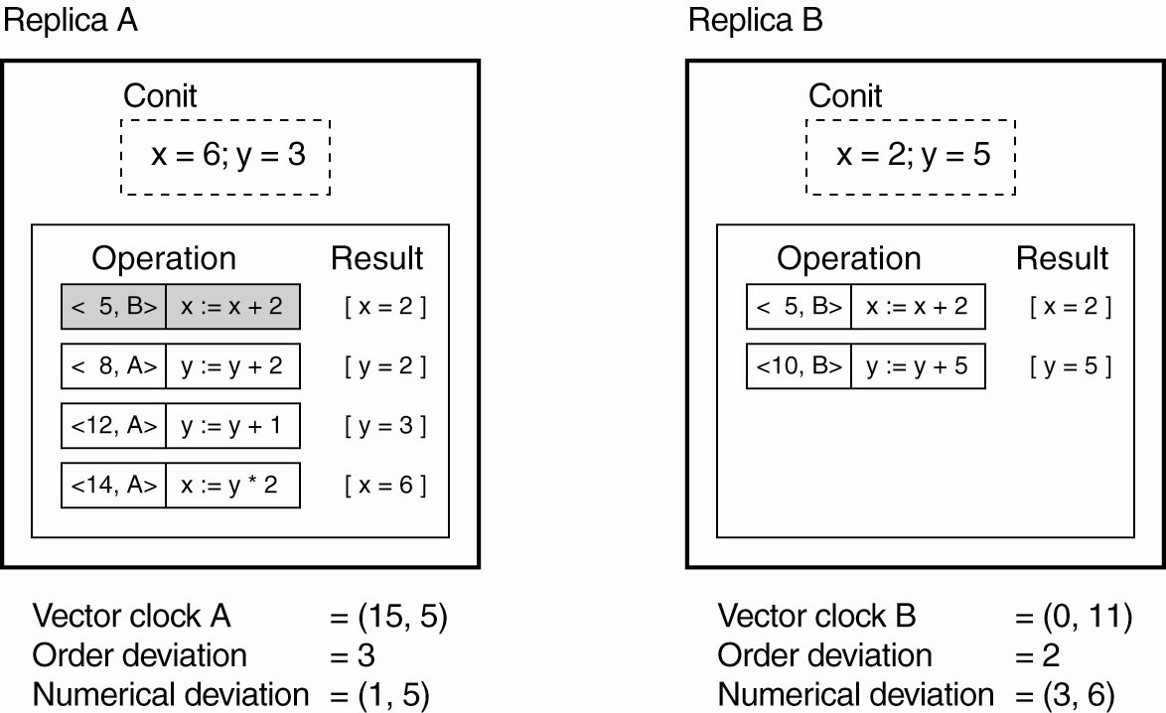
\includegraphics[width=\textwidth]{Media/ConitSample.jpg}
    \end{figure}
    Replica $A$ recieved the operation $<5,B>x:=x+2$ from replica $B$ and has committed it.\\
    Replica $A$ also has three tentative update operations: $<8,A>,<12,A>$ and $<14,A>$, which brings it's ordering deviation to 3, A's vector clock becomes $<15,5>$ because the last operation $<14,A>$ is followed by an incrementation.\\
    The only operation from $B$ that $A$ has not yet seen is $<10,B>$, therefore it's numerical deviation with respect to operation is 1, the weight of the deviation can be expressed as the maximum difference between the committed values of $x$ and $y$ at $A$, and the result from operations at $B$ not seen by $A$. The committed value at $A$ is $(x,y)=(2,0)$ whereas the for $A$ unseen-operation at $B$ yields a difference of $y=5$, therefore the Numerical deviation for $A$ is $(1,5)$\\
    \\
    \textbf{Similarly} for $B$. It has two tentative update operations: $<5,B>$ and $<10,B>$, which means it has an order deviation of $2$. Because $B$ has not yet seen a single operation from $A$, it's vector clock is $(0,11)$. The numerical deviation is 3, with a total weight of 6, because $B$'s committed value is: $(x,y)=(0,0)$, whereas the tentative operations at $A$ will bring $x$ to $6$.
    
    \chapter{Sequential consistency}
    A data store is said to be sequentially consistent when it satisfies the following condition:\\
    \\
    When processes run concurrently on (possibly) different machines, any valid interleaving of read and write operations is acceptable behaviour, but \textit{all processes must see the same interleaving of operations.}
    \begin{figure}[H]
	    \centering
	    \begin{subfigure}[b]{0.475\textwidth}
	        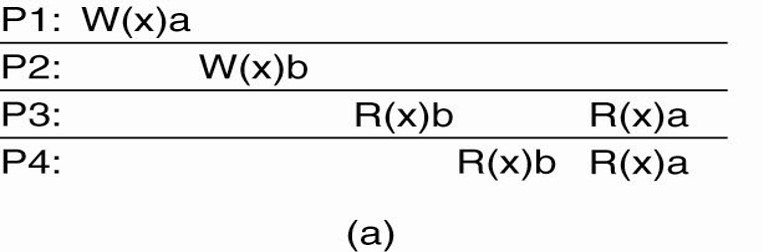
\includegraphics[width=\textwidth]{Media/Sequ1.jpg}
	    \end{subfigure}
	    \begin{subfigure}[b]{0.475\textwidth}
	        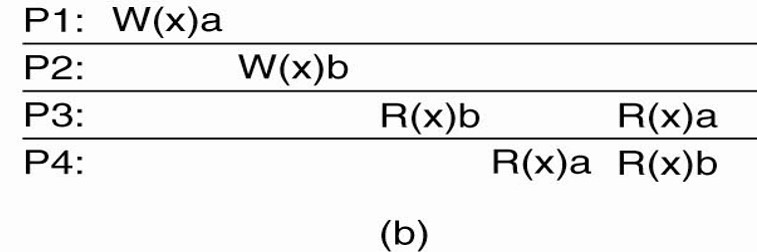
\includegraphics[width=\textwidth]{Media/Sequ2.jpg}
	    \end{subfigure}
	\end{figure}
	(a) is valid because all processes see the same interleaving, while (b) is not because $P3$ and $P4$ see different interleavings, ending up with different values for $x$.
	
	\chapter{Causal consistency}
	Much like sequential consistency, but only for potentially causally related events.

    \begin{figure}[H]
    \centering
    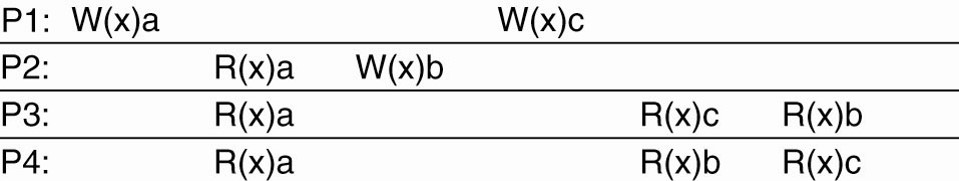
\includegraphics[width=\textwidth]{Media/Causal1.jpg}
    \end{figure}
    These events are causally consistent but not sequentially consistent, because $W(x)c$ and $W(x)b$ are concurrent (i.e. not causally related).
    \begin{figure}[H]
	    \centering
	    \begin{subfigure}[b]{0.475\textwidth}
	        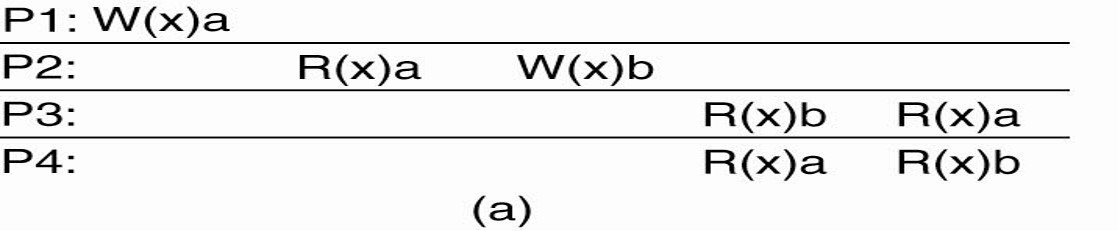
\includegraphics[width=\textwidth]{Media/Causal2.jpg}
	    \end{subfigure}
	    \begin{subfigure}[b]{0.475\textwidth}
	        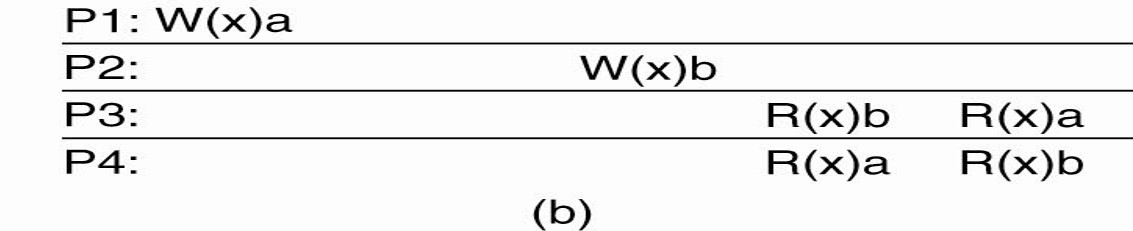
\includegraphics[width=\textwidth]{Media/Causal3.jpg}
	    \end{subfigure}
   	\end{figure}
   	Here (a) is not causally consistent because $R(x)a$ and $W(x)b$ is causally related, but (b) is causally consistent because we removed $R(x)a$ so it doesn't matter that $P3$ and $P4$ is reading $a$ and $b$ in a different order.
\end{document}